%2multibyte Version: 5.50.0.2953 CodePage: 1252

\documentclass[bigger,handout]{beamer}
%%%%%%%%%%%%%%%%%%%%%%%%%%%%%%%%%%%%%%%%%%%%%%%%%%%%%%%%%%%%%%%%%%%%%%%%%%%%%%%%%%%%%%%%%%%%%%%%%%%%%%%%%%%%%%%%%%%%%%%%%%%%%%%%%%%%%%%%%%%%%%%%%%%%%%%%%%%%%%%%%%%%%%%%%%%%%%%%%%%%%%%%%%%%%%%%%%%%%%%%%%%%%%%%%%%%%%%%%%%%%%%%%%%%%%%%%%%%%%%%%%%%%%%%%%%%
\usepackage{amssymb}
\usepackage{amsfonts}
\usepackage{amsmath}
\usepackage{mathpazo}
\usepackage{hyperref}
\usepackage{multimedia}
\usepackage{graphicx}

\setcounter{MaxMatrixCols}{10}
%TCIDATA{OutputFilter=LATEX.DLL}
%TCIDATA{Version=5.50.0.2953}
%TCIDATA{Codepage=1252}
%TCIDATA{<META NAME="SaveForMode" CONTENT="1">}
%TCIDATA{BibliographyScheme=Manual}
%TCIDATA{Created=Monday, October 27, 2008 15:56:24}
%TCIDATA{LastRevised=Thursday, April 27, 2017 21:53:27}
%TCIDATA{<META NAME="GraphicsSave" CONTENT="32">}
%TCIDATA{<META NAME="DocumentShell" CONTENT="Other Documents\SW\Slides - Beamer">}
%TCIDATA{Language=American English}
%TCIDATA{CSTFile=beamer.cst}

\newenvironment{stepenumerate}{\begin{enumerate}[<+->]}{\end{enumerate}}
\newenvironment{stepitemize}{\begin{itemize}[<+->]}{\end{itemize} }
\newenvironment{stepenumeratewithalert}{\begin{enumerate}[<+-| alert@+>]}{\end{enumerate}}
\newenvironment{stepitemizewithalert}{\begin{itemize}[<+-| alert@+>]}{\end{itemize} }
\usetheme{Madrid}
\usecolortheme{beaver}
\usefonttheme{professionalfonts}
\input{tcilatex}
\setbeamertemplate{navigation symbols}{}
\begin{document}

\title[47-809: Functional Eq's]{Functional equations}
\subtitle{Judd Chapters 10,11}
\author[David Childers]{David Childers (thanks to Y. Kryukov, K. Judd, and U. Doraszelski)}
\institute[CMU]{CMU, Tepper School of Business}
\date[Apr.5]{April 5, 2023}
\maketitle

\section{Functional equations}

 
 
\begin{frame}%
  
\frametitle{The Plan: building methods for dynamic problems}

\begin{itemize}
\item In dynamic problems, the unknown is often a function

\begin{itemize}
\item Dynamic Programming: Value and policy as function of state

\item Optimal Control: State and policy as function of time
\end{itemize}

\item Differential equations \& finite difference method

\begin{itemize}
\item ODE: $y^{\prime }\left( x\right) =f\left( y\left( x\right) ,x\right) $

\item Finite difference method: build a spline approximation to $y$ recursively

\item Econ. problems are optimization; one way to derive an ODE is Optimal
Control approach (Hamiltonian conditions)
\end{itemize}

\item Projection methods

\begin{itemize}
\item Global function approximation

\item Coefficients approximately solve any conditions on the function,\newline
e.g. the Bellman equation of Dynamic programming
\end{itemize}

\item Optimal Control will be covered in a later class
\end{itemize}

  
 
\end{frame}%
  
 
 
\begin{frame}%
  
\frametitle{Motivation}

\begin{itemize}
\item Optimal growth -- social planner solves:%
\begin{equation*}
\begin{array}{rc}
\max_{c} & \int_{0}^{\infty }e^{-\rho t}u\{c(t)\}dt \\ 
\text{subject to:} & \dot{k}\equiv k^{\prime }(t)=f\{k(t)\}-c(t) \\ 
& k(0)=\bar{k}_{0}%
\end{array}%
\end{equation*}

\begin{itemize}
\item $u(c)=\frac{c^{\gamma +1}}{\gamma +1}$ is the utility function

\item $f(k)=Ak^{\alpha }$ is the production function.
\end{itemize}

\item Opt.Control: derive $c^{\prime }(t)\equiv \dot{c}$ from optimality
conditions,\newline
so $C^{\prime }\left( k\right) =\dot{c}/\dot{k}$ is an ODE

\begin{itemize}
\item Today's ODE: assume $c\left( t\right) =\left( 1-s\right) f(k\left(
t\right)) $, so $k^{\prime }(t)=sf\{k(t)\}$
\end{itemize}

\item Dynamic progamming: solve Bellman equation \newline
for for $C\left( k\right) $ and $V\left( k\right) $.
\end{itemize}

  
 
\end{frame}%
  
 
 
\begin{frame}%
  
\frametitle{Ordinary Differential Equation (ODE)}

\begin{stepitemize}
\item First-order ODE: 
\begin{equation*}
\frac{dy}{dx}=f(y,x),
\end{equation*}%
where $f:R^{n+1}\rightarrow \mathbb{R}^{n}$ is the known function\newline
and $y:[a,b]\subset \mathbb{R}\rightarrow \mathbb{R}^{n}$ is the unknown
solution.

\item A $k$th order ODE can be transformed into a system of $k$ first-order
ODEs. 
\begin{equation*}
\frac{d^{2}y}{dx^{2}}=f(\frac{dy}{dx},y,x)\Leftrightarrow \left\{ 
\begin{array}{c}
\frac{dy}{dx}=z \\ 
\frac{dz}{dx}=f(z,y,x)%
\end{array}%
\right\}
\end{equation*}

\item Initial value problem (IVP) -- conditions on the solution \newline
at a single point: 
\begin{equation*}
y(x_{0})=y_{0},
\end{equation*}

\item Boundary value problem (BVP) -- at several points: 
\begin{equation*}
g_{i}(y(x_{i}))=0,\qquad i=1,\ldots ,n
\end{equation*}
\end{stepitemize}

  
 
\end{frame}%
  
 
 
\begin{frame}%
  
\frametitle{Linear ODE-IVP}

\begin{itemize}
\item If the problem is linear in $y^{\prime }$ and $y$:%
\begin{eqnarray*}
y^{\prime }\left( x\right) +a\left( x\right) y &=&b\left( x\right) , \\
y\left( 0\right) &=&y_{0}
\end{eqnarray*}

\item There is a closed-form solution:%
\begin{eqnarray*}
y\left( x\right) &=&y_{0}\exp \left\{ -\int_{0}^{x}a\left( s\right)
ds\right\} + \\
&&+\int_{0}^{x}\exp \left\{ -\int_{0}^{s}a\left( r\right) dr\right\} b\left(
s\right) ds
\end{eqnarray*}

\item Constant coefficients simplify the problem:%
\begin{eqnarray*}
y^{\prime }\left( x\right) &=&Ay,y\left( 0\right) =y_{0} \\
&\Rightarrow &y\left( x\right) =y_{0}\exp \left\{ Ax\right\}
\end{eqnarray*}
\end{itemize}

  
 
\end{frame}%
  
 
 
\begin{frame}%
  
\frametitle{General IVP: Euler methods}

IVP: $y^{\prime }(x)=f(y(x),x)$, $y(x_{0})=y_{0}$; $y:\left[ a,b\right]
\rightarrow \mathbb{R}$, $x_{0}=a$

\begin{stepitemize}
\item Grid $x_{i}=x_{0}+ih$, where $i=0,1,\ldots ,N$ and $h=\frac{b-a}{N}$.

\item Goal: Find $Y_{i}=\widehat{y(x_{i})}$
\end{stepitemize}

\textbf{Explicit Euler method}:

\begin{stepitemize}
\item Taylor approximation of $y$ around $x_{i}$, evaluated at $x_{i+1}$: 
\begin{equation*}
y(x_{i+1})\approx y(x_{i})+y^{\prime }(x_{i})(x_{i+1}-x_{i})
\end{equation*}

\item Recall that $x_{i+1}-x_{i}=h$, and compute:%
\begin{equation}
Y_{i+1}=Y_{i}+hf(Y_{i},x_{i}),\quad Y_{0}=y_{0}  \tag{EE}
\end{equation}

\item Straightforward computation ($i=1,...,N$)

\item If $y\in C^{3}[a,b]$, $f\in C^{2}$, and $f_{y}$ and $f_{yy}$ are
bounded, \newline
then error of Euler method shrinks in proportion to $h$.
\end{stepitemize}

  
 
\end{frame}%
  
 
 
\begin{frame}%
  
\frametitle{Implicit Euler method}

\begin{stepitemize}
\item Same approximation, but around $x_{i+1}$ \& evaluated at $x_{i}$:%
\begin{equation*}
y(x_{i})\approx y(x_{i+1})+y^{\prime }(x_{i+1})(x_{i}-x_{i+1})
\end{equation*}

\item Again, $x_{i}-x_{i+1}=-h$ and solve: 
\begin{equation}
Y_{i+1}=Y_{i}+hf(Y_{i+1},x_{i+1})  \tag{IE}
\end{equation}

\item (IE) is a nonlinear equation in $Y_{i+1}$ $\Rightarrow $ slower step

\begin{itemize}
\item Implement as Newton's method at each $i$,

\item or as a fixed-point iteration (need $\left\vert hf_{y}\right\vert <1$),

\item or as a large system of nonlinear equations.
\end{itemize}

\item More stable $\Rightarrow $ can use higher $h$ $\Rightarrow $ less steps

\item Both Euler methods assume $y^{\prime }(x)$ is a step-function, \newline
so $y(x)$ is piecewise linear
\end{stepitemize}

  
 
\end{frame}%
  
 
 
\begin{frame}%
  
\frametitle{Trapezoid method}

\begin{stepitemize}
\item Combine explicit and implicit Euler:%
\begin{equation}
Y_{i+1}=Y_{i}+\frac{h}{2}\left[ f(Y_{i},x_{i})+f(Y_{i+1},x_{i+1})\right] 
\tag{T}
\end{equation}

\item Assumes $y^{\prime }(x)$ is piecewise linear,

\item so $y(x)$ is piecewise quadratic.

\item Convergence is quadratic: error $\sim h^{2}$

\item Method is also implicit since (T) defines $Y_{i+1}$ \newline
as the solution to an equation.\bigskip

\item Runge-Kutta scheme generalizes finite difference methods:

\begin{equation*}
Y_{i+1}=Y_{i}+\frac{h}{2}\left[ f(Y_{i},x_{i})+f(Y_{i}+hf(x_i,Y_i),x_{i+1})\right] 
\end{equation*}
\begin{stepitemize}
\item Also quadratic, but explicit
\end{stepitemize}
\end{stepitemize}

  
 
\end{frame}%
  
 
 
\begin{frame}%
  
\frametitle{Runge-Kutta 4th order scheme}

\begin{equation*}
Y_{i+1}=Y_{i}+\frac{h}{6}\left[ z_{1}+2z_{2}+2z_{3}+z_{4}\right] ,\quad
Y_{0}=y_{0},
\end{equation*}%
where 
\begin{eqnarray*}
z_{1} &=&f(Y_{i},x_{i}), \\
z_{2} &=&f(Y_{i}+\frac{h}{2}z_{1},x_{i}+\frac{h}{2}), \\
z_{3} &=&f(Y_{i}+\frac{h}{2}z_{2},x_{i}+\frac{h}{2}), \\
z_{4} &=&f(Y_{i}+hz_{3},x_{i}+h).
\end{eqnarray*}

\begin{itemize}
\item Explicit

\item Converges at rate $h^{4}$.

\item Each step evaluates $f$ four times.
\end{itemize}

  
 
\end{frame}%
  
 
 
\begin{frame}%
  
\frametitle{Example: constant growth rate}

\begin{itemize}
\item Growth model with constant savings rate $s$:%
\begin{gather*}
\dot{k}\equiv k^{\prime }(t)=sf\{k(t)\}, \\
k\left( 0\right) =\bar{k}_{0}
\end{gather*}

\item 1st order ODE,

\begin{itemize}
\item nonlinear if $f\left( \cdot \right) $ is nonlinear

\item IVP: $k\left( 0\right) =\bar{k}_{0}$
\end{itemize}

\item Grid over the argument of the function: $t_{i}=ih$

\item Runge-Kutta: Compute $k_{i+1}=\widehat{k\left( t_{i+1}\right) }$ using $k_{i}$
and $t_{i+1}$
\end{itemize}

  
 
\end{frame}%
  
 
 
\begin{frame}%
  
\frametitle{Boundary value problem (BVP)}

General form (with two point conditions): 
\begin{gather*}
\dot{x}(t)=f(x(t),y(t),t),\quad x(0)=\bar{x}_{0}, \\
\dot{y}(t)=g(x(t),y(t),t),\quad y(T)=\bar{y}_{T}.
\end{gather*}

Solution = \textbf{Shooting}

\begin{stepitemize}
\item Initialization: Guess $y_{0}$ and choose stopping criterion $\epsilon $%
.

\item Step 1: Solve the IVP 
\begin{gather*}
\dot{x}(t)=f(x(t),y(t),t),\quad x(0)=\bar{x}_{0}, \\
\dot{y}(t)=g(x(t),y(t),t),\quad y(0)=y_{0}.
\end{gather*}

\begin{itemize}
\item Let $Y(T,y^{0})$ be the resulting approximation for $y(T)$.
\end{itemize}

\item Step 2: If $||Y(T,y^{0})-\bar{y}_{T}||<\epsilon $, stop; otherwise, 
\newline
adjust $y_{0}$ -- using Bisection, Secant, etc. \medskip

\item I.e. solve the nonlinear equation $Y(T;y^{0})=\bar{y}_{T}$.
\end{stepitemize}

  
 
\end{frame}%
  
 
 
\begin{frame}%
  
\frametitle{BVP example: Life-cycle consumption}

\begin{itemize}
\item Consumer with lifespan $T$ solves:%
\begin{equation*}
\begin{array}{rc}
\max_{c} & \int_{0}^{T}e^{-\rho t}u(c)dt \\ 
\text{subject to} & \dot{A}=f(A)+w-c, \\ 
& A(0)=A(T)=0%
\end{array}%
\end{equation*}

\begin{itemize}
\item $A(t)$ = assets that consumer holds at time $t$

\item $w$ = wage, $f\left( \cdot \right) $ = return on investment
\end{itemize}

\item Optimal Control methods (Hamiltonian + Pontryagin conditions, topic 9)
tell us that:%
\begin{eqnarray*}
\dot{c} &=&\frac{u^{\prime }(c)}{u^{\prime \prime }(c)}\left( \rho
-f^{\prime }(A)\right) , \\
\dot{A} &=&f(A)+w-c
\end{eqnarray*}

\item Shooting: pick $c\left( 0\right) $ to make $A\left( T\right) =0$
(Fig.10.2)
\end{itemize}

  
 
\end{frame}%

\begin{frame}
\scalebox{0.5}{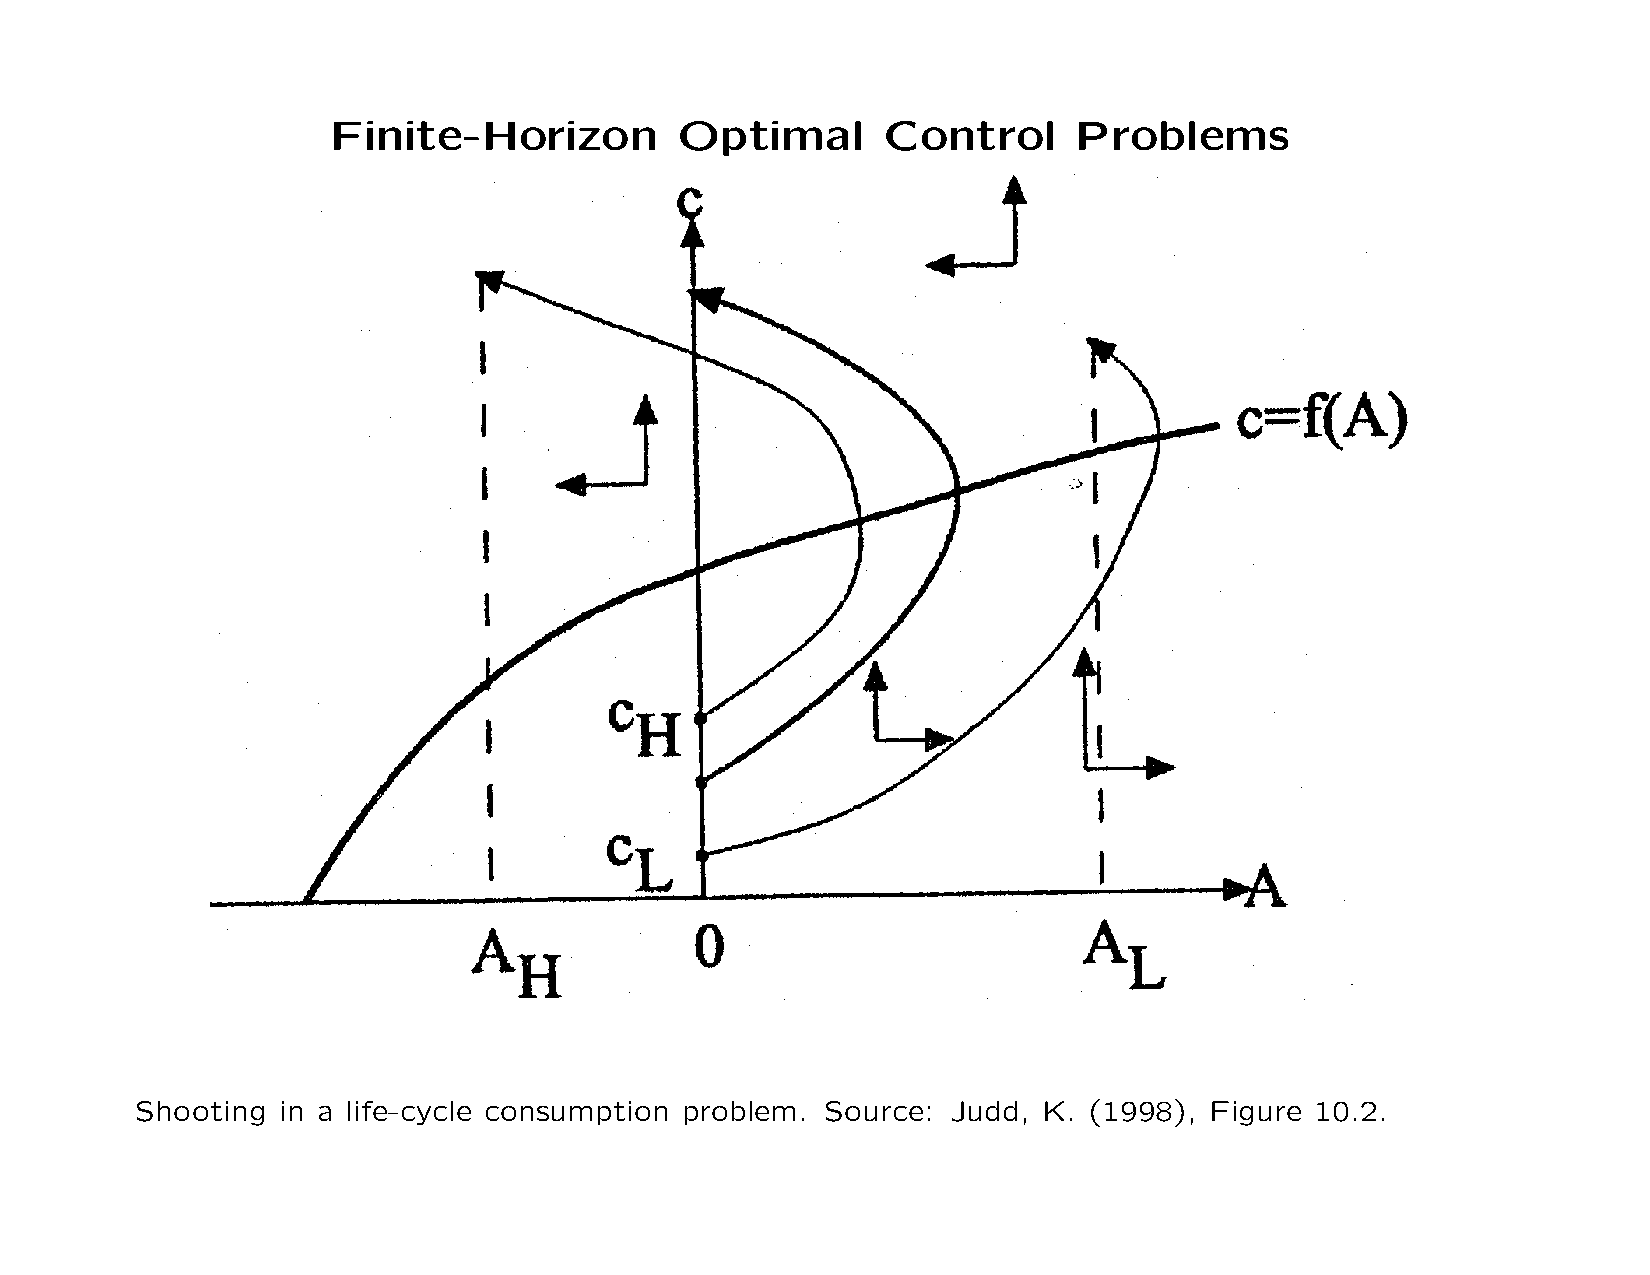
\includegraphics{shootingmethod.pdf}}

\end{frame}
  
 
 
\begin{frame}%
  
\frametitle{Projection: idea}

\begin{itemize}
\item Solving $y^{\prime }(x)=f(y(x),x)$, $y\left( 0\right) =y_{0}$, for $%
x\in \lbrack 0,\bar{X}]$

\item Finite difference methods construct $y\left( \cdot \right) $ from splines

\item Projection chooses function representation to minimize global measure of error
\begin{equation*}
\hat{y}\left( x\right) =y_{0}+\tsum\nolimits_{j=1}^{n}a_{j}\phi _{j}\left(
x\right)
\end{equation*}

\begin{itemize}
\item $a_{0}\equiv y_{0}$ to fit the initial condition (here, $\phi
_{j}\left( 0\right) \equiv 0$)
\end{itemize}

\item Define function operator: $\left[ \mathcal{L}y\right] \left( x\right) =%
\left[ y^{\prime }(x)-f(y(x),x)\right] \left( x\right) $

\item Solution $y^{\ast }\left( \cdot \right) $ must satisfy $\left[ 
\mathcal{L}y^{\ast }\right] \left( x\right) =0$, $\forall x\in \left[ 0,\bar{%
X}\right] $

\item Idea: find coefficients $a$ that make $\mathcal{L}\hat{y}\left(
x\right) $ "small",

\begin{itemize}
\item To this end, define \textbf{residual function}: 
\begin{equation*}
R\left( x;a\right) \equiv \mathcal{L}\hat{y}\left( x\right)
=\tsum\nolimits_{j=1}^{n}a_{j}\phi _{j}^{\prime }\left( x\right)
-f(y_{0}+\tsum\nolimits_{j=1}^{n}a_{j}\phi _{j}\left( x\right) ,x)
\end{equation*}
\end{itemize}
\end{itemize}

  
 
\end{frame}%
  
 
 
\begin{frame}%
  
\frametitle{Projection: approaches}

\begin{itemize}
\item Want to find $a$ that makes $R\left( x;a\right)=\mathcal{L}\left[\sum_{j=1}^{n}a_j\phi_j\right](x) $ small
\item Different approaches use different function representation, different def of "small"
\item \emph{Spectral} methods solve exactly $\left\langle R(x,a),\psi_i(x)\right\rangle=0$ $\forall i$

\begin{itemize}
\item $n$ unknowns ($a$) $\Rightarrow $ need $n$ equations
\item Representation should approximate solution well
\item Choose $\psi$ to approximate range space well
\item Use knowledge of function class (differentiable, etc)
\end{itemize}

\item Finding $a$: solve system of $n$ equations
\begin{itemize}
\item If $\mathcal{L}$ and $\hat{y}$ linear, system is linear
\item Otherwise, use nonlinear solution method: e.g. fixed point, Newton
\end{itemize}
\item Warning: $\frac{d}{da}\mathcal{L}$ can be very badly conditioned
\begin{itemize}
\item E.g. $\mathcal{L}=\int_{s}^{t}k(x,z)\hat{y}(z)dz=0$ Fredholm eq of 1st kind
\item $\to$ use penalized method
\end{itemize}

\end{itemize}
 
\end{frame}%


\begin{frame}%

\frametitle{Spectral approaches: examples}

\begin{itemize}

\item \emph{Galerkin}: Use $\left\{\psi\right\}$ an orthonormal basis

\begin{itemize}
\item Typically: $\left\{\psi\right\}=\left\{\phi\right\}$ orthogonal polynomials
\item Can differentiate, integrate exactly in many cases
\item \emph{Petrov-Galerkin} $\left\{\psi\right\}\neq\left\{\phi\right\}$
\item o.n.b. ensures $L^2$ approx of input and output
\item Exponentially fast approximation in $n$ \emph{if} solution known to be smooth
\end{itemize}


\item \emph{Least squares}:%
\begin{equation*}
\min_{a}\int_{0}^{\bar{X}}\left[ R\left( x;a\right) \right] ^{2}dx
\end{equation*}

\begin{itemize}
\item FOC's: one equation for each $a_{j}$: $\left\langle R(x,a),\frac{\partial}{da_{j}}R(x,a)\right\rangle=0$
\item Special case solvable by optimization
\end{itemize}

\end{itemize}


\end{frame}%



\begin{frame}%
  
\frametitle{Pseudo-spectral approaches}

\begin{itemize}

\item Spectral methods: evaluate $R(x,a)$ and inner products
\begin{itemize}
\item Need closed form for operator \emph{and} integral
\end{itemize}
\item Instead, can approximate inner product by quadrature
\item If $\mathcal{L}$ itself involves integral, use quadrature here too
\begin{equation*}
\int\int k(x,z)\sum_{j=1}^{n}a_{j}\phi_{j}(z)dz\psi_{i}(x)dx=\sum_{j=1}^{n}a_{j}\left\langle k(x,z),\phi_{j}\psi_{i}\right\rangle
\end{equation*}

\item Choose quadrature method to fit function choice
\begin{itemize}
\item Gaussian or other exact method for polynomials
\end{itemize}

\item (Chebyshev) \emph{Collocation}: pick $n$ nodes $x_{i}$, and solve:%
\begin{equation*}
R\left( x_{i};a\right) =0,\qquad i=1,...,n
\end{equation*}

\begin{itemize}
\item Nodes $x_{i}$ = degree $n$ Chebyshev points, mapped into $\left[ 0,\bar{X}\right] $
\item $\phi _{j}\left( x\right) $ any basis, $\psi_j$ are \emph{implicitly} Chebyshev polynomials
\item Uses interpolation (fast) in place of exact projection (slow)
\end{itemize}

\end{itemize}
 
\end{frame}%  
 
 
\begin{frame}%
  
\frametitle{Projection: applications}

\begin{itemize}

\item If solving a system of ODE's:

\begin{itemize}
\item Separate approximation for each univariate function

\item Separate residual f-n for each eq-n $\Rightarrow $ same number of nodes
\end{itemize}

\item If solving BVP: need to account for boundary conditions
\item Either add as equation $\hat{y}(x_0)=a_0$
\item or choose basis that satisfies for all $a$: "solve out"

\item Projection method works for all functional equations, \newline
not just ODE's:

\begin{itemize}
\item Bellman $\Rightarrow $ eq's in terms of value and policy functions

\item Optimal control approach: ODE for policy function\newline
(with steady state as the "initial" value)

\item Euler equation: eq-n in terms of policy function (next slide)
\end{itemize}
\end{itemize}
  
 
\end{frame}%
  
 
 
\begin{frame}%
  
\frametitle{Projection example: Euler equation}

\begin{itemize}
\item Discrete-time growth model:%
\begin{eqnarray*}
&&\max_{c,k}\tsum\nolimits_{t=1}^{\infty }\beta ^{t}u\left( c_{t}\right) \\
\text{s.t.} &:&k_{t+1}=f\left( k_{t}\right) -c_{t}
\end{eqnarray*}

\item Substitute $c_{t}=f\left( k_{t}\right) -k_{t+1}$, take FOC w.r.t. $%
k_{t+1}$:%
\begin{equation*}
u^{\prime }\left( c_{t}\right) =\beta u^{\prime }\left( c_{t+1}\right)
f^{\prime }\left( k_{t+1}\right)
\end{equation*}

\item Rewrite in terms of policy function: $c_{t}=C\left( k_{t}\right) $:%
\begin{equation*}
\mathcal{L}C\left( k\right) \equiv \left[ 
\begin{array}{l}
u^{\prime }\left[ C\left( k\right) \right] \\ 
-\beta u^{\prime }\left[ C\left( f\left( k\right) -C\left( k\right) \right) %
\right] f^{\prime }\left( f\left( k\right) -C\left( k\right) \right)%
\end{array}%
\right] =0
\end{equation*}

\item Apply $\mathcal{L}$ to $\hat{C}\left( k;a\right)
=\tsum\nolimits_{j=0}^{n}a_{j}\phi _{j}\left( k\right) :$%
\begin{equation*}
R\left( k;a\right) \equiv \mathcal{L}\hat{C}\left( k;a\right)
\end{equation*}
\end{itemize}

  
 
\end{frame}%
  
 
 
\begin{frame}%
  
\frametitle{Projection implementation}

\begin{itemize}
\item Need a good non-linear equation solver, or optimizer

\begin{itemize}
\item Note that there is no coefficient regression anymore
\end{itemize}

\item Starting values of coefficients are often crucial

\begin{itemize}
\item Set low-degree coefficients to correct slope and curvature

\item Leave higher-order coefficients at zero
\end{itemize}

\item Plot resulting function and residuals

\begin{itemize}
\item Function: Check slope and curvature; \newline
reduce degree of polynomials if too many waves

\item Residuals: make sure they are small everywhere; \newline
increase degree if there is bias in their sign
\end{itemize}

\item Code polynomial evaluation as a separate function

\begin{itemize}
\item Or pre-compute polynomials at nodes
\end{itemize}
\end{itemize}

  
 
\end{frame}%


\begin{frame}%
  
\frametitle{Projection Pros and Cons}

\begin{itemize}
\item When solution well-approximated by known basis, can be really accurate
\begin{itemize}
\item Error can decay exponentially in $n$ if $y(.)$ analytic
\item Guarantees depend on "well-posedness" of $\mathcal{L}$
\item Combine with analytical results to ensure good behavior
\end{itemize}
\item Requires solving system: 
\begin{itemize}
\item If linear, up to $O(n^3)$, if nonlinear, $O(n^3)$ each iteration 
\end{itemize}
\item Finite difference methods effectively solve system also, but due to locality get sparsity, fast $O(n)$ solves
\item Big gains to using structure for faster system solves, integrals
\item Advanced function representation can help:
\begin{itemize}
\item Adaptive methods: add new basis/node using residuals
\item Neural nets, Smolyak can be applied if dimension large
\end{itemize}
\item Choice often depends on needs in rest of multistep algorithm
\begin{itemize}
\item May need continuity or other function property
\end{itemize}



\end{itemize}

\end{frame}%

\begin{frame}%
  
\frametitle{References}

\begin{itemize}
\item Ordinary Differential Equations
\begin{itemize}
\item SciML \href{https://book.sciml.ai/}{Book}, \href{https://docs.sciml.a}{Docs}, \href{https://github.com/SciML/SciMLTutorials.jl}{Tutorials} 
\end{itemize}
\item Projection:
\begin{itemize}
\item \href{https://depts.washington.edu/ph506/Boyd.pdf}{Boyd: Chebyshev and Fourier Spectral Methods}
\item \href{https://epubs.siam.org/doi/book/10.1137/1.9781611970678}{Chatelin: Spectral Approximation of Linear Operators}
\item Econ-specific: Fern\'{a}ndez-Villaverde et al Macro Handbook
\end{itemize}
\end{itemize}


\end{frame}%
  
 
%  
% \begin{frame}%
%   
% \frametitle{Example: Bellman with cont. state}
% 
% \begin{itemize}
% \item Original problem:%
% \begin{equation*}
% V(x)=\max_{u}\pi (x,u)+\beta \int V(x^{+})dF(x^{+},x,u)
% \end{equation*}
% 
% \item Compute FOC:%
% \begin{equation*}
% 0=\pi _{u}(x,u)+\beta \int V(x^{+})dF_{u}(x^{+},x,u)
% \end{equation*}
% 
% \item If FOC is sufficient, optimal $V(x)$ and $U(x)$ must satisfy: 
% \begin{gather*}
% V(x)=\pi (x,U(x))+\beta \int V(x^{+})dF(x^{+},x,U(x)), \\
% 0=\pi _{u}(x,U(x))+\beta \int V(x^{+})dF_{u}(x^{+},x,U(x)).
% \end{gather*}
% \end{itemize}
% 
%   
%  
% \end{frame}%
%   
%  
%  
% \begin{frame}%
%   
% \frametitle{Example: Bellman with cont. state}
% 
% Solving for unknown $V(\cdot )$ and $U(\cdot )$
% 
% \begin{itemize}
% \item Set up polynomial approximation $\hat{V}(x;a)$ and $\hat{U}(x;b)$
% 
% \begin{itemize}
% \item Degree $N$ approximations $\Rightarrow \ \left\{ a,b\right\} \in 
% \mathbb{R}^{2(N+1)}$
% \end{itemize}
% 
% \item Pick $N+1$ nodes $x_{i}$ -- e.g. polynomial roots
% 
% \item System of equations$,$ $i=1:N+1:$%
% \begin{eqnarray*}
% -\hat{V}(x_{i})+\pi (x_{i},\hat{U}(x_{i}))+\beta \int \hat{V}%
% (x^{+})dF(x^{+},x_{i},\hat{U}(x_{i})) &=&0 \\
% \pi _{u}(x_{i},\hat{U}(x_{i}))+\beta \int \hat{V}(x^{+})dF_{u}(x^{+},x_{i},%
% \hat{U}(x_{i})) &=&0
% \end{eqnarray*}
% 
% \begin{itemize}
% \item where $\hat{V}(x)\equiv \hat{V}(x;a)$, $\hat{U}(x)\equiv \hat{U}(x;b)$
% 
% \item Variables: $\left\{ a,b\right\} \in \mathbb{R}^{2(N+1)}$
% \end{itemize}
% \end{itemize}
% 
%   
%  
% \end{frame}%
%   
 
 
% \begin{frame}%
%   
% \frametitle{Summary of methods}
% 
% All problems that deal with functions are based on two main approaches of
% representing them:\bigskip
% %%% NO NO NO NO NO: This view is really misleading
% 
% \begin{tabular}{|l|l|l|}
% \hline
% $y\left( x\right) $ & Piecewise & Global polynomials \\ \hline
% f-n representation & Spline & Orth. Polynomial \\ 
% Integration & Newton-Coates & Quadrature \\ 
% Functional eq-ns & ODE R-K schemes & Projection \\ \hline
% \end{tabular}
% 
%   
%  
% \end{frame}%
  

\end{document}


